% Muc 4.2  --  phu trach: Hùng
% nguon: docs/system_overview.md §7 (tang 1-8); python/dsp/pan_tompkins.py (docstring: chuyen 200 -> 360 Hz, nguong);
%        python/quant/pipeline_int.py (loc, tinh chinh R, cua so, z-score, RR so nguyen); python/dsp/filters.py (Butterworth);
%        NHATKY.md cua repo 1DCNN (Se/+P detector DS1); trung vi dac trung RR: cache beats_annotation, 22 ban ghi DS1
\section{Tiền xử lý tín hiệu bằng số nguyên}\label{sec:tienxuly}

Khối tiền xử lý nhận tín hiệu MIT-BIH và cho ra tín hiệu đã lọc $y$ cùng vị trí đỉnh R của từng nhịp, là đầu vào của khối trích xuất đặc trưng ở Mục~\ref{sec:dactrung}.
Mọi bộ lọc đều nhân quả để hệ thống xử lý được tín hiệu theo thời gian thực, và mọi phép tính là số nguyên để phần cứng cài đặt lại vẫn khớp từng bit với mô hình tham chiếu.
Huấn luyện và triển khai dùng chung khối này.

Hình~\ref{fig:tienxuly} trình bày các khối xử lý chính: dữ liệu MIT-BIH đi qua tiền xử lý, trích xuất đặc trưng, mô hình CNN, lượng tử hoá, đánh giá và cuối cùng là xuất dữ liệu; mô hình được trình bày ở Mục~\ref{sec:cnnlite} và Mục~\ref{sec:huanluyen}, lượng tử hoá ở Mục~\ref{sec:luongtu}.
Khối tiền xử lý gồm hai nhánh song song.
Nhánh phát hiện chỉ cần biết nhịp nằm ở đâu, nên được phép làm biến dạng tín hiệu để mỗi phức bộ QRS thành một đỉnh nổi bật.
Nhánh hình dạng phải giữ hình dạng thật của nhịp cho mạng phân loại, nên chỉ lọc nhẹ.
Hình~\ref{fig:ch4-khoitienxuly} bóc tách khối tiền xử lý thành các khâu, và Bảng~\ref{tab:ch4-tienxuly} tóm tắt phép toán và độ trễ của từng khâu.

\begin{figure}[htbp]
  \centering
  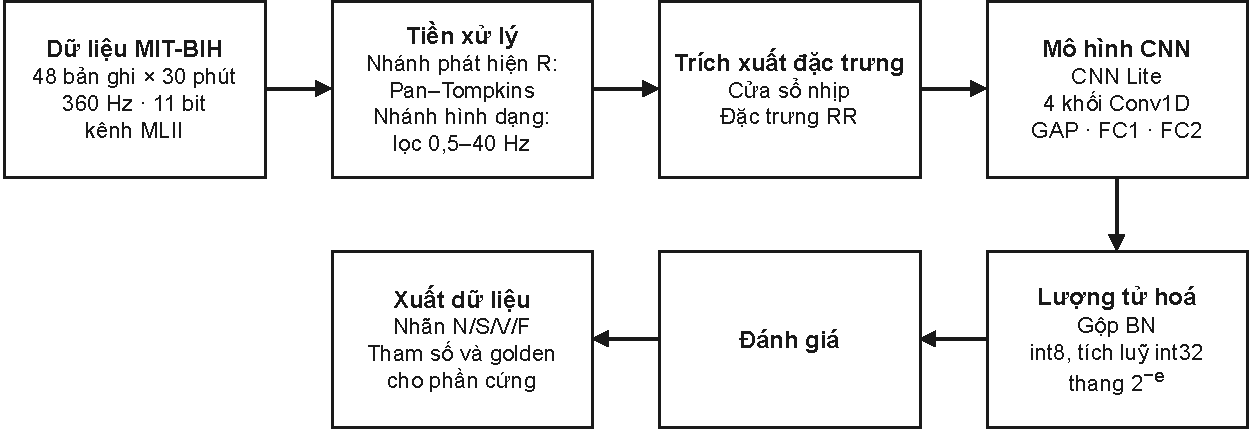
\includegraphics[width=\textwidth]{ch04_mo_hinh_cnn/luong_tong}
  \caption{Các khối xử lý chính của phần mô hình, từ dữ liệu MIT-BIH đến dữ liệu xuất ra.}\label{fig:tienxuly}
\end{figure}

\begin{figure}[htbp]
  \centering
  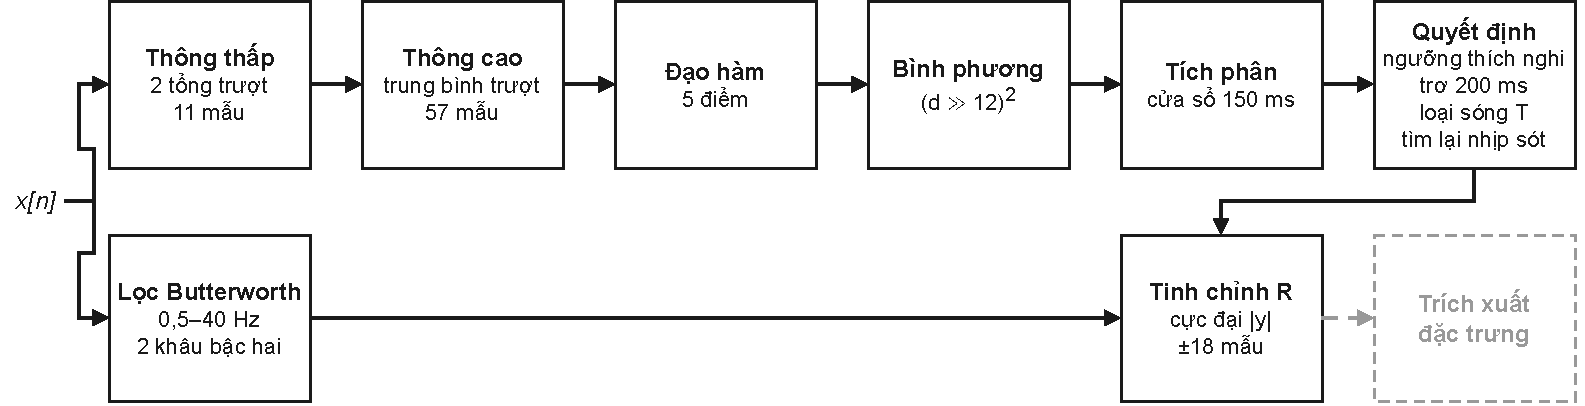
\includegraphics[width=\textwidth]{ch04_mo_hinh_cnn/khoi_tienxuly}
  \caption{Các khâu của khối tiền xử lý: nhánh phát hiện R (hàng trên) và nhánh hình dạng (hàng dưới); khối nét đứt là khối kế tiếp.}\label{fig:ch4-khoitienxuly}
\end{figure}

\begin{table}[htbp]
  \centering
  \caption{Tóm tắt các khâu tiền xử lý số nguyên.}\label{tab:ch4-tienxuly}
  \small\setlength{\tabcolsep}{4pt}
  \begin{tabular}{@{}llll@{}}
    \toprule
    Khâu & Phép toán chính & Đầu ra & Độ trễ \\
    \midrule
    \multicolumn{4}{@{}l}{\emph{Nhánh phát hiện}} \\
    Thông thấp + thông cao & tổng trượt 11, 11 và 57 mẫu & tín hiệu dải 5--12\,Hz & 38 mẫu \\
    Đạo hàm, bình phương & sai phân 5 điểm, dịch 12 bit, nhân & năng lượng sườn dốc & 2 mẫu \\
    Tích phân cửa sổ & tổng trượt 54 mẫu & một đỉnh cho mỗi QRS & 26{,}5 mẫu \\
    Quyết định & ngưỡng thích nghi, dịch bit & vị trí R thô & 0{,}21--0{,}32\,s \\
    \midrule
    \multicolumn{4}{@{}l}{\emph{Nhánh hình dạng}} \\
    Lọc 0{,}5--40\,Hz & 2 khâu bậc hai, hệ số $2^{20}$ & tín hiệu đã lọc & 2 mẫu \\
    Tinh chỉnh R & tìm cực đại trong $\pm18$ mẫu & vị trí R & 0 \\
    \bottomrule
  \end{tabular}
\end{table}

\subsection{Nhánh phát hiện}

Mỗi bản ghi MIT-BIH lưu sẵn các mẫu số nguyên $u[n]$ 11 bit, điểm không ở 1024, 200 đơn vị trên mỗi mV.
Trước hết tín hiệu được đưa về dao động quanh 0:
\begin{equation}
  x[n]=u[n]-1024,\qquad |x[n]|\le2^{10}.
  \label{eq:ch4-adc}
\end{equation}
Biết trước $|x|\le2^{10}$ nên tính được giá trị lớn nhất ở mỗi khâu sau và kiểm được rằng không khâu nào tràn số nguyên 32 bit.

Nhánh phát hiện dùng thuật toán Pan--Tompkins~\cite{pantompkins1985realtime}.
Bản gốc thiết kế cho 200\,Hz; ở 360\,Hz, mọi độ dài và khoảng thời gian được nhân $1{,}8$ rồi làm tròn.
Các phép chia chuẩn hoá của bản gốc được bỏ đi, vì chúng chỉ đổi thang tín hiệu còn các ngưỡng phía sau tự thích nghi theo biên độ.
Năm khâu của nhánh là:
\begin{align}
  \mathrm{lp}[n]&=\sum_{k=0}^{10}s[n-k],\quad s[n]=\sum_{k=0}^{10}x[n-k], \label{eq:ch4-lp}\\
  \mathrm{hp}[n]&=57\cdot\mathrm{lp}[n-28]-\sum_{k=0}^{56}\mathrm{lp}[n-k], \label{eq:ch4-hp}\\
  d[n]&=2\,\mathrm{hp}[n]+\mathrm{hp}[n-1]-\mathrm{hp}[n-3]-2\,\mathrm{hp}[n-4], \label{eq:ch4-der}\\
  q[n]&=\big(d[n]\gg12\big)^{2}, \label{eq:ch4-sq}\\
  \mathrm{mwi}[n]&=\sum_{k=0}^{53}q[n-k]. \label{eq:ch4-mwi}
\end{align}
\begin{itemize}
  \item \textbf{Thông thấp} \eqref{eq:ch4-lp}: hai tổng trượt dài 11 mẫu (bản gốc dài 6) nối tiếp, cho đáp ứng xung hình tam giác và loại nhiễu tần cao.
  \item \textbf{Thông cao} \eqref{eq:ch4-hp}: tín hiệu trễ trừ trung bình trượt của chính nó, chỉ còn lại phần biến đổi nhanh.
  Độ dài 57 (bản gốc 32) là số lẻ để độ trễ 28 mẫu là số nguyên; nhân số hạng trễ với 57 thay cho chia tổng cho 57.
  Hai khâu lọc tạo thành bộ thông dải 4{,}9--11{,}8\,Hz ở mức $-3$\,dB, là dải chứa phần lớn năng lượng QRS, với tổng độ trễ 38 mẫu.
  \item \textbf{Đạo hàm} \eqref{eq:ch4-der}: công thức năm điểm của bản gốc, bỏ hệ số $1/8$, làm nổi bật sườn dốc của QRS so với sóng P và T.
  \item \textbf{Bình phương} \eqref{eq:ch4-sq}: đưa mọi giá trị về dương và khuếch đại sườn dốc; dịch 12 bit trước để kết quả vừa 32 bit.
  \item \textbf{Tích phân} \eqref{eq:ch4-mwi}: cửa sổ 54 mẫu bằng 150\,ms, xấp xỉ độ rộng QRS, gộp mỗi phức bộ thành một đỉnh; giá trị lớn nhất $2^{29{,}3}$ vẫn nhỏ hơn $2^{31}$.
\end{itemize}

Khối quyết định xếp mỗi đỉnh của $\mathrm{mwi}$ vào loại nhịp hoặc nhiễu.
Theo bản gốc, khối giữ mức đỉnh nhịp $\mathrm{SPK}$ và mức đỉnh nhiễu $\mathrm{NPK}$, cập nhật mỗi khi có một đỉnh cao $p$, rồi suy ra hai ngưỡng:
\begin{equation}
  \begin{gathered}
  \mathrm{SPK}\leftarrow\mathrm{SPK}+\big((p-\mathrm{SPK})\gg3\big),\\
  \mathrm{THR1}=\mathrm{NPK}+\big((\mathrm{SPK}-\mathrm{NPK})\gg2\big),\qquad
  \mathrm{THR2}=\mathrm{THR1}\gg1,
  \end{gathered}
  \label{eq:ch4-thr}
\end{equation}
với $\mathrm{NPK}$ cập nhật giống $\mathrm{SPK}$.
Công thức gốc $\mathrm{SPK}\leftarrow0{,}125\,p+0{,}875\,\mathrm{SPK}$ được viết lại thành dịch phải 3 bit, cho kết quả như nhau trên số nguyên mà không cần phép nhân.
$\mathrm{THR1}$ nằm ở một phần tư khoảng từ mức nhiễu lên mức nhịp, nên tự thích ứng khi biên độ thay đổi giữa các bệnh nhân.
Một đỉnh là nhịp khi vượt ngưỡng trên cả $\mathrm{mwi}$ và tín hiệu thông dải.
Khối áp dụng thêm ba quy tắc sinh lý: bỏ qua mọi đỉnh trong 200\,ms sau một nhịp vì cơ tim chưa thể co lại; coi đỉnh trong vòng 360\,ms có độ dốc nhỏ hơn một nửa nhịp trước là sóng T; nếu sau $1{,}66$ lần RR trung bình chưa có nhịp thì tìm lại với ngưỡng $\mathrm{THR2}$, trong đó $1{,}66$ được xấp xỉ bằng $1+\tfrac12+\tfrac18+\tfrac1{32}$.

Hình~\ref{fig:ch4-pt} cho thấy tín hiệu qua các khâu trên một đoạn có nhịp N xen nhịp V.
Sau thông dải chỉ còn dao động quanh QRS; sau tích phân mỗi QRS là một đỉnh rộng, và $\mathrm{THR1}$ nằm dưới đỉnh của cả hai loại nhịp nên không nhịp nào bị bỏ sót.
Trên DS1, bộ phát hiện đạt độ nhạy 99{,}633\,\% và độ chính xác dương 99{,}146\,\%.

\begin{figure}[htbp]
  \centering
  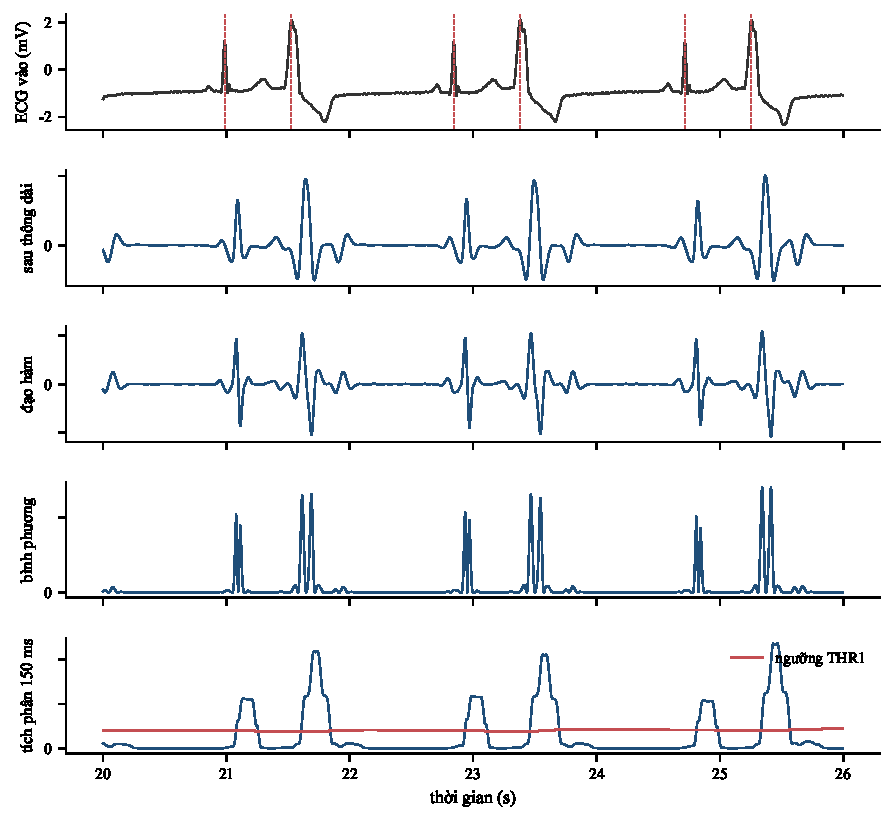
\includegraphics[width=\textwidth]{ch04_mo_hinh_cnn/pt_cackhau.pdf}
  \caption{Tín hiệu qua các khâu Pan--Tompkins số nguyên trên 6\,s của bản ghi 119 (DS1). Đường đứt nét ở hàng trên là vị trí R được phát hiện; đường đỏ ở hàng dưới là ngưỡng thích nghi $\mathrm{THR1}$.}\label{fig:ch4-pt}
\end{figure}

\subsection{Nhánh hình dạng}

\paragraph{Lọc thông dải.}
Bộ lọc Butterworth 0{,}5--40\,Hz loại trôi đường nền do hô hấp, cử động (dưới 0{,}5\,Hz) và nhiễu cơ, nhiễu điện lưới (trên 40\,Hz), nhưng vẫn giữ sóng P, QRS và T.
Butterworth có dải thông phẳng nên không làm méo biên độ tương đối giữa các sóng; bậc thấp cho ít hệ số và ổn định khi làm tròn.
Bộ lọc gồm hai khâu bậc hai nối tiếp, mỗi khâu tính theo
\begin{equation}
  y[n]=b_0x[n]+b_1x[n-1]+b_2x[n-2]-a_1y[n-1]-a_2y[n-2].
  \label{eq:ch4-biquad}
\end{equation}
Khâu thứ nhất có tử số $(1+z^{-1})^2$, triệt tần cao; khâu thứ hai có tử số $(1-z^{-1})^2$, triệt thành phần một chiều.
Trên số nguyên, hệ số được nhân $2^{20}$, tín hiệu được nhân $2^{12}$, tổng tính trên 64 bit rồi đổi thang bằng $y=(\mathrm{acc}+2^{19})\gg20$; sai lệch so với bộ lọc số thực khoảng 0{,}1\,\%.
Hệ số cụ thể ở Phụ lục~\ref{pl:luongtu}.

\paragraph{Tinh chỉnh R.}
Vị trí R thô $r_c$ lấy từ tín hiệu đã biến dạng nên có thể lệch vài mẫu; nó được dời về điểm có biên độ tuyệt đối lớn nhất trong $\pm50$\,ms của tín hiệu đã lọc $y$:
\begin{equation}
  R=\underset{|r-r_c|\le18}{\arg\max}\;\big|y[r+D]\big|,
  \label{eq:ch4-refine}
\end{equation}
với $D=2$ là độ trễ của bộ lọc.
Trị tuyệt đối giúp tìm đúng đỉnh cả khi QRS hướng xuống, như ở nhiều nhịp V.
